% USAGE: copy contents of this file into ourApproach.tex


\section{Our Approach}
\subsection{Data Description}
Our data set is a collection of 476 million tweets from 17 million unique users spanning from June 2009 to December 2009 collected by Stanford University through their partnership with Twitter. We limit this data set to 178 million tweets during July and August in order to save on computation costs for our clustering and classification.

We first perform several preprocessing steps to prepare the data for clustering. We remove all tweets containing non-ASCII characters in order to focus on English-language content.  From the resulting set, we remove the tweets that contain no hashtags, which leaves around 16 million tweets. We remove all non-alphanumeric characters, resulting in a list of hashtags and non-hashtag \emph{terms} (i.e. words, numbers) used in each tweet.  The resulting data set contains 872,402 hashtags.

It may seem worrisome that less than ten percent of the tweets in our subset contain a hashtag, and that we are basing much of our learning on the presence of hashtags. However, we still have more than enough data to detect patterns in. Furthermore, we see this as a potential application area for semi-supervised learning. Once a reliable method of predicting the hashtag content of a tweet is developed, the remaining 90 percent of tweets could be assigned hashtag labels to summarize their subject matter.

The final preprocessing step is to remove certain hashtags that are either auto-generated by external systems or are \emph{overly-general} hashtags, i.e. those whose usage is too broad to consider their co-occurence with other tags to be meaningful. For example, the hashtag $\#fb$  is automatically appended by a particular Facebook application that shares Facebook posts on Twitter. An example of an overly-general hashtag is $\#followfriday$, which is a hashtag used on Fridays to recommend other users to follow.

From this preprocessed data, we generate a list of the most frequently used hashtags, along with the co-occurrence frequencies of all hashtags with each other. We limit our data set to the most frequently occurring hashtags and the hashtags that they co-occur with in order to simplify the clustering problem.

\subsection{Clustering Hashtags}
\subsubsection{Difficulties of Clustering}
There are a number of variables that make it difficult to cluster hashtags. The first major difficulty is that hashtags are not required to be well-defined words. For example, the hashtag $\#p2$ is often used in tweets with politically progressive content. In many cases, hashtags are a concatenation of words like $\#iamthemob$.  

Some similarity measures like the Wu-Palmer distance and path distance are based on the synonyms of the words being examined, which means that they can't be used as central component in a clustering algorithm such as $k$-means. However, our algorithm will still use this concept in a more limited scope.

The fact that hashtags are often concatenations of words makes it difficult to apply the Levenshtein distance or other edit distances. For example, under edit distance the hashtags $\#iamblessed$ and $\#iamthemob$ are close to one another when in fact their semantic meanings are very different. We tried to implement a method using this distance, but it resulted in poor results.

The set of hashtags is constantly increasing in size, with new, ``trendy'' hashtags appearing everyday. Therefore we want to use an algorithm that captures the essence of the most-used hashtags, while remaining computationally tractable. We decided to focus clustering on the 2,000 most frequently used hashtags. However, our algorithm does not discard the lesser-used hashtags; instead, it focuses its efforts on the most-used hashtags.

\subsubsection{Co-Occurrence Relation}
Poschko proposes that two hashtags are similar if they co-occur in a tweet \cite{Poschko2011}. Two hashtags may be considered similar to each other if they appear in tweets that discuss the same topic, and are therefore even more similar if they appear within the same tweet. Poschko calculates the Wu-Palmer distance between hashtags that co-occur and shows that this value is higher than the distance between two randomly chosen words. Although the Wu-Palmer distance is a poor distance for hashtags as a whole because they often are not single words, it does provide a good measure over the set of hashtags only containing single words. We propose that because the Wu-Palmer distance is high for reoccurring hashtags that are real words, then the set of all reoccurring hashtags can be used as baseline for a similarity measure.

After creating the co-occurrence lists for the 2,000 most used hashtags, we used the Natural Language Toolkit (NLTK) Python library to find the Wu-Palmer distance for each hashtag in each list, then took the average over all of the lists. For hashtags that co-occur, this value was .40, and for random words it was .16. These results verify that the claim by Poschko applies to our data set: that the hashtags found in the co-occurrence list are much more similar to each other than random words are.
    
\subsubsection{Minimizing the Level of Noise}
Even though the list as a whole exhibits similarity, there is still noise in the data. For example, $\#photography$ is a popular hashtag used to denote a photograph, and another hashtag is often used within the same tweet to describe the place the picture was taken, such as $\#iran$. In this case, the fact that these hashtags co-occur does not mean that they are similar by our definition of similarity. To help minimize this problem, let $n_{ij}$ be the total number of co-occurrences between hashtag $i$ and hashtag $j$. Hashtags A and B are kept on the co-occurring list if and only if
\begin{eqnarray}
min (\frac{n_{AB}}{ \sum n_{Aj}}, \frac{n_{BA}} {\sum n_{Bj}}) > 0.05. \nonumber
\end{eqnarray}
This means that hashtags A and B account for at least 5$\%$ of each others co-occurring hashtags. Several different percentages were tested and this one provided the best results.

Noisy relationships still exists after this step. Therefore, we perform another round of filtering by comparing the contents of the hashtags' respective co-occurrence lists. Let $m$ be the total number of hashtags that occur in both hashtag A's and hashtag B's co-occurrence lists. Further, let $m_A$ be the total number of occurrences of these hashtags in list A, and $m_B$ be the total number of occurrences in list B. Then the relationship between hashtag A and hashtag B is maintained if an only if
\begin{eqnarray}
min (\frac{{m_A} }{\sum n_{Aj}}, \frac{m_B }{ \sum n_{Bj}} ) > 0.2. \nonumber
\end{eqnarray}
Note that by the first level of filtering, this minimum is at least 0.05. Comparing each list takes a considerable amount of time to run, and this bottleneck was a motivating factor in our decision to constrain our focus to only 2,000 hashtags. However, it is easily parallelizable, and when programmed efficiently could allow a much greater number of hashtags to be considered; we leave such optimizations for future work.

\subsubsection{Defining the Similarity Measure}
We define the following similarity measure between hashtags A and hashtags B:
\begin{eqnarray}
S(A,B) = ( \frac{n_{AB}}{\sum n_{Aj}} + \frac{n_{BA} } {\sum n_{Bj}}) /2 . \nonumber
\end{eqnarray}
It should be noted that several similarity measures were tested, such as multiplying the two ratios together, but this proved to be the best measure.

\begin{figure}[tbh]
\centering
\subfigure[]{
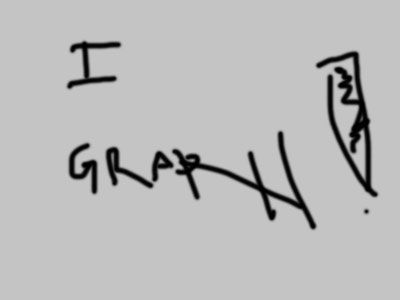
\includegraphics[scale=0.20]{./wordGraphs/slide1.jpg}
}
\subfigure[]{
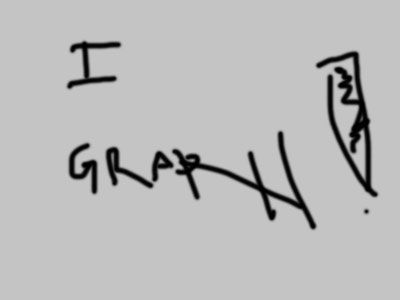
\includegraphics[scale=0.20]{./wordGraphs/slide2.jpg}
}
\subfigure[]{
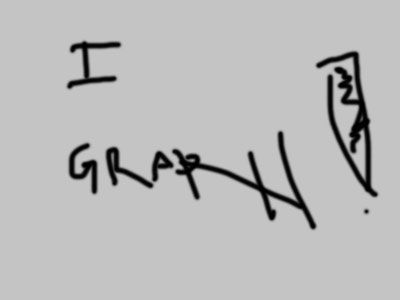
\includegraphics[scale=0.20]{./wordGraphs/slide3.jpg}
}
\subfigure[]{
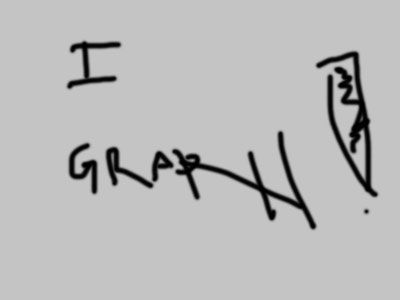
\includegraphics[scale=0.20]{./wordGraphs/slide4.jpg}
}
\subfigure[]{
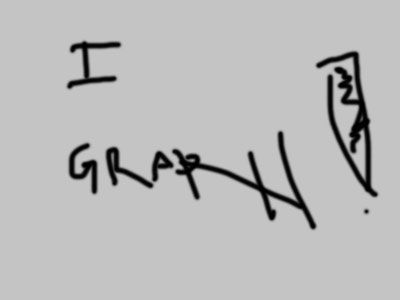
\includegraphics[scale=0.20]{./wordGraphs/slide5.jpg}
}
\subfigure[]{
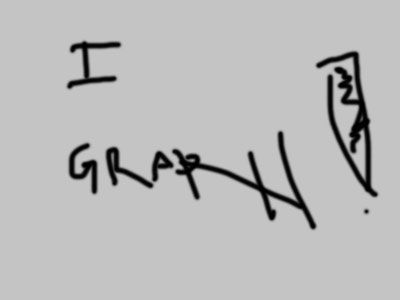
\includegraphics[scale=0.20]{./wordGraphs/slide6.jpg}
}
\caption{Subfigure (a) represents the original undirected graph proposed by the co-occurring lists. Subfigures (b) and (c) consist only of the neighbors of apple and iphone respectively (the graph remains undirected). Subfigures (d) and (e) convert the undirected graphs into an directed graph by weighing the edges. The filter process examines these directed graphs, and after passing the final undirected graph with the similarity measure is created (f).}
\label{fig:words}
\end{figure}

\subsubsection{Spectral Clustering and METIS}
With our well-defined similarity measure, and therefore a similarity matrix, spectral clustering was the ideal candidate to perform clustering over our list of hashtags. For comparison purposes, we performed spectral clustering and normalized spectral clustering. We also examined the graph program METIS that claimed to perform 10$\%$ to 50$\%$ better than spectral algorithms \cite{Karypis1998}. This algorithm is based on multilevel recursive-bisection and multilevel k-way partitioning schemes. Instead of using an Laplacian matrix like the spectral methods, METIS takes in the similarity matrix, and uses the similarity measures to define a weighted graph.

Even though these methods cluster over the 2,000 most used hashtags, we maintain the co-occurring lists with each of these hashtags. As a result, even the hashtags which are not in the top 2,000 are then assigned to a cluster. Referring back to Figure 1, if apple and iphone are clustered together, then mac, google, and app will appear in the same cluster. If a hashtag appears in more than one cluster, it is assigned to the one it occurs most frequently in. In all, 26,028 hashtags are clustered using the spectral methods and 26,006 are clustered using METIS.

\subsubsection{Expanding Clusters with Cosine Similarity Measure}
In order to expand the breadth of our clustering techniques, we optionally find unclustered tags that are textually very similar to a tag in an existing cluster, and then expand the cluster to include the previously-unclassified tag.

To determine the textual similarity of two tags, we first vectorize the tags and then take their cosine similarity. Our vectorization technique is similar to taking the character-wise trigram of a word, with a simplification in order to reduce the cost of computing the cosine of two vectors.

We represent each tag $t$ as a list of tokens with one token for each letter in the tag, plus an additional dummy token at the beginning of the list and one at the end of the list. The binary high-dimensional sparse representation $b$ of a tag, indexed using $i, j, k \in [1-38]$, is
\begin{eqnarray}
b(tag)_{i,j,k} = 1_{\{subseq(i, j, k) \in tag\}} \nonumber
\end{eqnarray}

In other words, each dimension in $b$ corresponds to a possible sequence of three characters; the corresponding value in $b$ is $1$ if that sequence of characters is in the list of tokens $l$, or $0$ otherwise. Restricting these values to $0$ or $1$ allows us to find the dot product of two vectors more quickly than allowing each dimension to take on  larger range of values. The cosine similarity between two binary vectors is the dot product of the two vectors divided by the product of the magnitudes of the vectors:

\begin{eqnarray}
cos(x, y) = \frac{ \sum_{i,j,k} 1_{\{ x_{i,j,k} = y_{i,j,k} = 1 \}} }{  \sqrt{\sum_j x_j^2} + \sqrt{ \sum_j y_j^2 }  } \nonumber
\end{eqnarray}

In order to pair an unclassified tag with an existing cluster, we find the clustered tag from the top 2,000 tags that it is most similar to. If their similarity is above the threshold $0.5$, we add the tag to the cluster. Otherwise, we leave the tag unclustered. Performing this additional hashtag-class assignment increases the number of tags assigned to any cluster from 26,028 to 52,146 under the spectral clustering methods, and from 26,006 to 52,032 under METIS.

\subsection{Classification}
\setcounter{secnumdepth}{4}

In the classification step, we attempt to classify tweets into classes defined by the hashtag clusters. Intuitively, the idea is that given the text of a tweet, the classification algorithms will be able to suggest what hashtags it should contain. Since we have actually clustered the hashtags, we will not be suggesting what hashtags the tweet will contain, but will suggest which cluster the hashtag is most likely to fall into.  

\subsubsection{Description of feature vectors and classes}
For classification, we have a corpus of text tweets that we will map to clusters of hashtags. We can consider each tweet a document and use standard document classification techniques in this step. We create a set of all unique words (removing common stopwords and all hashtags) that occur in all the tweets. Let us assume that there are {\it d} words in the dictionary.  
The feature vector is a {\it d}-dimensional integer-valued vector where the {\it $i^{th}$} entry in the vector represents the frequency in the tweet of the {\it i$^{th}$} word in the set.

The classes that each feature vector is classified into is represented by the hashtag clusters. A tweet belongs to a class if a hashtag appearing in the tweet is part of a certain cluster. When generating the training data, if a tweet has multiple hashtags, we consider that tweet to be a part of multiple classes so we add the same training point multiple times with different classes as the target. We do this since the text of a tweet is related to all the hashtags in the tweet.  

Due to the size of our training sets, each feature vector was an extremely-sparse high-dimensional vector. Due to the number of training samples and the high dimensionality of the vector, attempting to classify over the complete data was intractable on any machines that we had access to. To get around this problem, we used two solutions.

\subsubsection{Classification using Dimensionality Reduction}

We used the PCA tools from the Python library{\it scikit-learn} to reduce the dimensionality in our data. For our data set containing 100,000 tweets, we had approximately 46,000 dimensions. We reduced this to 100 dimensions using PCA. Once we reduced the number of dimensions, it was possible to apply standard classification algorithms to the data. We applied Naiver Bayes and Linear Discriminant Analysis the to the reduced-dimension data.

Naive Bayes initially performed poorly because PCA creates real-valued feature vectors whose values don't always mean much. Instead, we used skikit-learn's implementation of Bernoulli naive Bayes, which binarizes the data by replacing all positive values in the feature vector with the value 1 and all negative values with the value 0. This performed much better than the other naive Bayes implementations. LDA performed acceptably well on the dimension-reduced data without the need to create a binary representation of the data.

\subsubsection{Classification using SVM algorithm optimized for sparse vectors}
An alternative approach to deal with the high dimensionality of our feature vectors is to use an algorithm that was designed to use the sparse representation of a vector. By representing the feature vectors as a sparse vector, the problem becomes tractable and we don't need to do any dimensionality reduction. We used scikit-learn's implementation of a radial basis SVM classifier, which supports sparse data represenatations. We use a one-versus-all strategy to make SVM a multi-class classifier. We also perform SVM classification on the PCA-reduced data.

\subsubsection{Majority Vote classification}
We determine the majority vote classification accuracy to use as a baseline measure. The majority vote accuracy is defined as the percentage of data points whose class label is the most common class label.